\documentclass{beamer}
\usetheme{Madrid}
\usecolortheme{default}
\usepackage[utf8]{inputenc}
\usepackage{tikz}
\usepackage{circuitikz}
\usepackage{enumitem}
\usepackage{array}
\usepackage{float}
\usepackage{amsmath}
\usepackage{subcaption}
\usepackage[export]{adjustbox}
\usetikzlibrary{arrows,shapes,automata,petri,positioning,calc}
\usetikzlibrary{positioning,shapes.gates.logic.US}

\colorlet{beamer@blendedblue}{green!60!black}
%\usebackgroundtemplate{\includegraphics[width=\paperwidth,height=\paperheight]{img/assn11_bg.png}} 

\tikzset{ 
    place/.style={
        circle,
        thick,
        draw=black,
        fill=gray!50,
        minimum size=6mm,
    },
        state/.style={
        circle,
        thick,
        draw=blue!75,
        fill=blue!20,
        minimum size=6mm,
    },
}

\title{Assignment 11}
\subtitle{Solution to gate EC 2014-2,question 9}


\AtBeginSection[]
{
  \begin{frame}
    \frametitle{Table of Contents}
    \tableofcontents[currentsection]
  \end{frame}
}

\begin{document}

\begin{frame}{}
    \maketitle
\end{frame}

\section{Question}

\begin{frame}{Question}
       The state transition diagram for the logic circuit shown as
\begin{figure}[h]
    \centering
    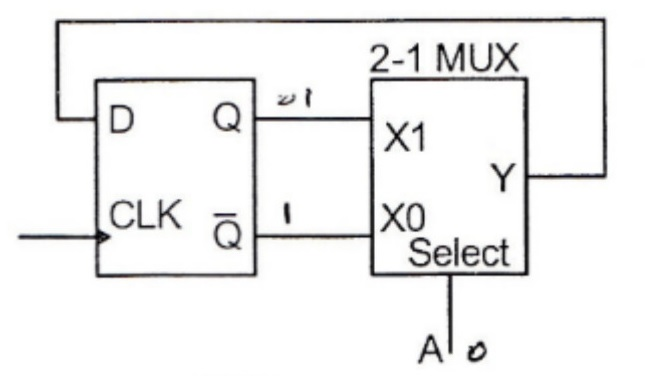
\includegraphics[width=0.4\textwidth]{images/QUES.jpg}
\end{figure}
 
\begin{figure}[H]
    \centering
    \begin{subfigure}[h]{0.4\textwidth}
        \scalebox{0.4}{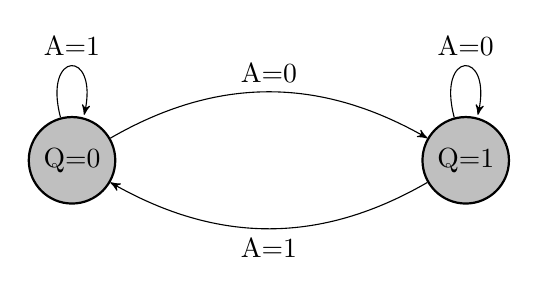
\begin{tikzpicture}[node distance=5cm and 4cm,>=stealth',auto, every place/.style={draw}]
    \node [place] (Q0) {Q=0};
    \coordinate[node distance=4cm,left of=Q0] (left-Q0);
    \coordinate[node distance=4cm,right of=Q0] (right-Q0);
    \node [place] (Q1) [right of=Q0] {Q=1};
    \path[->] (Q0) edge [bend left] node {A=0} (Q1);
    \path[->] (Q1) edge [loop above] node {A=0} (Q1);
    \path[->] (Q1) edge [bend left,] node {A=1} (Q0);
    \path[->] (Q0) edge [loop above] node {A=1} (Q0);
\end{tikzpicture}
 }
        \caption{(A)}
    \end{subfigure}
    \hfill
    \begin{subfigure}[h]{0.4\textwidth}
        \scalebox{0.4}{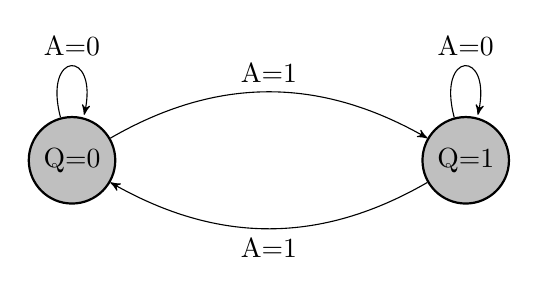
\begin{tikzpicture}[node distance=5cm and 4cm,>=stealth',auto, every place/.style={draw}]
    \node [place] (Q0) {Q=0};
    \coordinate[node distance=4cm,left of=Q0] (left-Q0);
    \coordinate[node distance=4cm,right of=Q0] (right-Q0);
    \node [place] (Q1) [right of=Q0] {Q=1};
    \path[->] (Q0) edge [bend left] node {A=1} (Q1);
    \path[->] (Q1) edge [loop above] node {A=0} (Q1);
    \path[->] (Q1) edge [bend left,] node {A=1} (Q0);
    \path[->] (Q0) edge [loop above] node {A=0} (Q0);
\end{tikzpicture}
 }
        \caption{(B)}
    \end{subfigure}
    \hfill
    \begin{subfigure}[h]{0.4\textwidth}
        \scalebox{0.4}{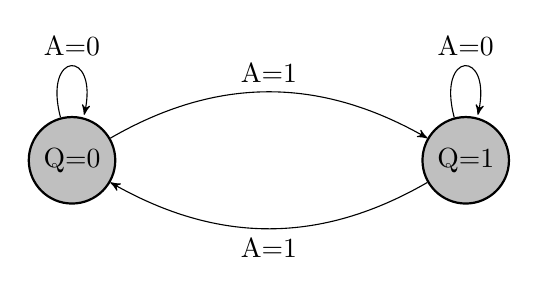
\begin{tikzpicture}[node distance=5cm and 4cm,>=stealth',auto, every place/.style={draw}]
    \node [place] (Q0) {Q=0};
    \coordinate[node distance=4cm,left of=Q0] (left-Q0);
    \coordinate[node distance=4cm,right of=Q0] (right-Q0);
    \node [place] (Q1) [right of=Q0] {Q=1};
    \path[->] (Q0) edge [bend left] node {A=1} (Q1);
    \path[->] (Q1) edge [loop above] node {A=0} (Q1);
    \path[->] (Q1) edge [bend left,] node {A=1} (Q0);
    \path[->] (Q0) edge [loop above] node {A=0} (Q0);
\end{tikzpicture}
 }
        \caption{(C)}
    \end{subfigure}
    \hfill    
     \begin{subfigure}[h]{0.4\textwidth}
        \scalebox{0.4}{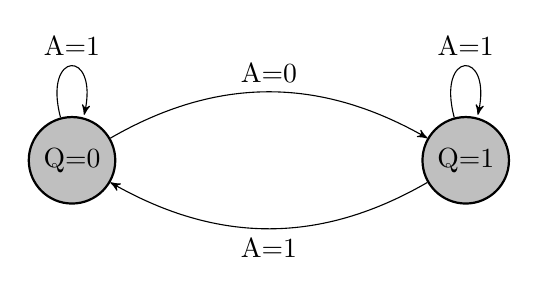
\begin{tikzpicture}[node distance=5cm and 4cm,>=stealth',auto, every place/.style={draw}]
    \node [place] (Q0) {Q=0};
    \coordinate[node distance=4cm,left of=Q0] (left-Q0);
    \coordinate[node distance=4cm,right of=Q0] (right-Q0);
    \node [place] (Q1) [right of=Q0] {Q=1};
    \path[->] (Q0) edge [bend left] node {A=0} (Q1);
    \path[->] (Q1) edge [loop above] node {A=1} (Q1);
    \path[->] (Q1) edge [bend left,] node {A=1} (Q0);
    \path[->] (Q0) edge [loop above] node {A=1} (Q0);
\end{tikzpicture}
 }
        \caption{(D)}
    \end{subfigure}
\end{figure}
\end{frame}

\section{Explanation}
\begin{frame}{Explanation}


    We know,
  
  2-1 MUX $\Longrightarrow$ 2-1 Multiplexer
  
  When   A=0,
  
  X$_0$   line  is  selected  and  connected  to $\overline{Q}$  and now  $\overline{Q}$
 
 is  now  connected  to  X$_0$  that  is,  X$_0$  is  going  to  be   shortened to  Y.  The
 
 output  Y  is  now  communicated  with  X$_0$  which  is  connected  to $\overline{Q}$.
  
  so,Y will become  whenever A=0
  
    $ Y=X_0=\overline{Q}=D$
     
    $ then,Q+  =\overline{Q}$
    
    and  similarly  when  A=1
    
    Y=X$_1$=Q=D
   Assume   that  Q=0  as one  state and Q=1  as another state
   
   At  state Q=0
   
    if  A=0
    
    then transition of state changes from Q=0 to Q=1
    
    if A=1
    
    then transition of state remains constant
    

\end{frame}

\begin{frame}{Explanation}
       At  state  Q=1
   
    if  A=0
    
    then transition of state remains constant
    
    if A=1
    
    then transition of state changes from Q=1 to Q=0
\end{frame}

    \section{State Transition}  
    
\begin{frame}{Transition Table}

  \begin{table}[h]
   \centering
   \begin{tabular}{|c|c|c|}
   \hline
   \textit{\textbf{Q (P.S) }}&\textit{\textbf{input D}} &\textbf{(N.S)$Q_n$} \\ \hline
    0 & 0    &  0     \\ \hline
    0 & 1    &  1     \\ \hline
    1 & 0    &  0     \\\hline
    1 & 1    &  1     \\ \hline
    \hline
   \end{tabular}
  \caption{Sate Transition Table }
\label{tab:table1}
\end{table}
\end{frame}

\section{Conclusion}
\begin{frame}{Conclusion}
     Hence  OPTION 'D' IS THE RIGHT OPTION
    
\begin{figure}[h]
    \centering
    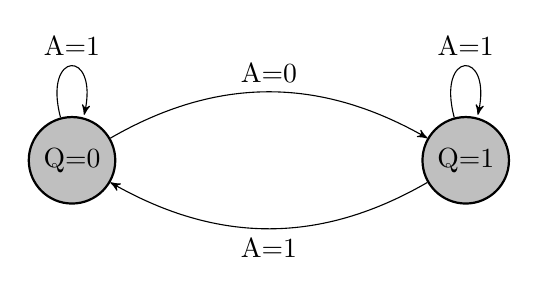
\begin{tikzpicture}[node distance=5cm and 4cm,>=stealth',auto, every place/.style={draw}]
    \node [place] (Q0) {Q=0};
    \coordinate[node distance=4cm,left of=Q0] (left-Q0);
    \coordinate[node distance=4cm,right of=Q0] (right-Q0);
    \node [place] (Q1) [right of=Q0] {Q=1};
    \path[->] (Q0) edge [bend left] node {A=0} (Q1);
    \path[->] (Q1) edge [loop above] node {A=1} (Q1);
    \path[->] (Q1) edge [bend left,] node {A=1} (Q0);
    \path[->] (Q0) edge [loop above] node {A=1} (Q0);
\end{tikzpicture}
 
\end{figure}
\end{frame}

\end{document}
